\section{Intuition}
The definition of homology groups is a little abstract, so in this section, we provide some intuition behind why is it defined the way it is.

To study a topological object, we can consider the set of loops on the object, identifying two loops to be equivalent if we can deform one loop into another. This is a very natural mathematical structure to study.

We can reformulate the equivalence relation between loops from a different point of view. Suppose we have two loops, labeled $A$ and $B$, as shown:
\begin{figure}[H]
    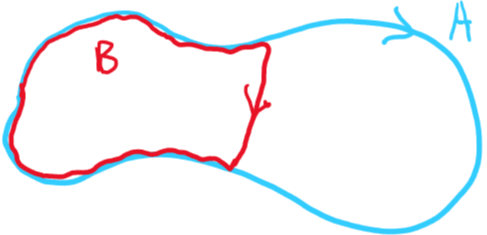
\includegraphics[width=5cm]{figures/intuition-1}
    \centering
\end{figure}
The loops $A$ and $B$ are equivalent (i.e. can be deformed into one another) if and only if the region $C$ shown below has no ``holes":
\begin{figure}[H]
    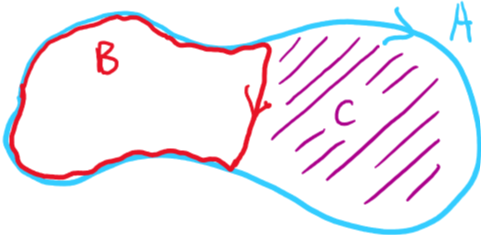
\includegraphics[width=5cm]{figures/intuition-2}
    \centering
\end{figure}
As $C$ has no holes, one possible oriented boundary of $C$, denoted $\partial C$, is:
\begin{figure}[H]
    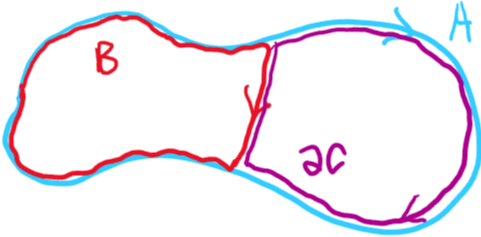
\includegraphics[width=5cm]{figures/intuition-3}
    \centering
\end{figure}
Note if we ``add" loop $B$ and loop $\partial C$, the oppositely oriented segments cancel out, and we get loop $A$:
\begin{figure}[H]
    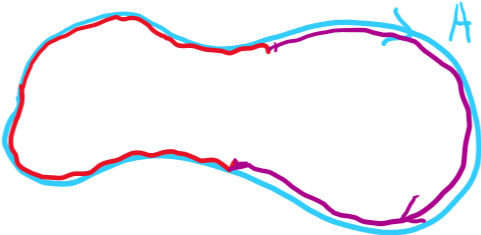
\includegraphics[width=5cm]{figures/intuition-4}
    \centering
\end{figure}
To summarize: loops $A$ and $B$ are equivalent if they ``differ" by the oriented boundary of some 2D region (which in this case is $C$). This observation turns out to be true with more complicated examples (although the region might no longer be a single connected component).

In the coming section, we will see the following definitions:
\begin{itemize}
    \item \textbf{$q$-cycle}: a $q$-dimensional loop
    \item \textbf{$q$-boundary}: a $q$-dimensional (oriented) boundary
    \item \textbf{$q$-th homology group}: the group of $q$-cycles, identifying two cycles to be equal if they ``differ" by a $q$-boundary
\end{itemize}
In other words, the $q$-th homology group can be thought as the set of $q$-dimensional loops (endowed with some group structure), identifying two loops to be equivalent if we can deform one loop into another.